\documentclass[border=10pt]{standalone}

\usepackage{tikz}
\usepackage{tikzsymbols}
\usetikzlibrary{calc,patterns,shapes.geometric}

\def\centerarc[#1](#2)(#3:#4:#5){\draw[#1] ($(#2)+({#5*cos(#3)},{#5*sin(#3)})$) arc (#3:#4:#5);}

\begin{document}
	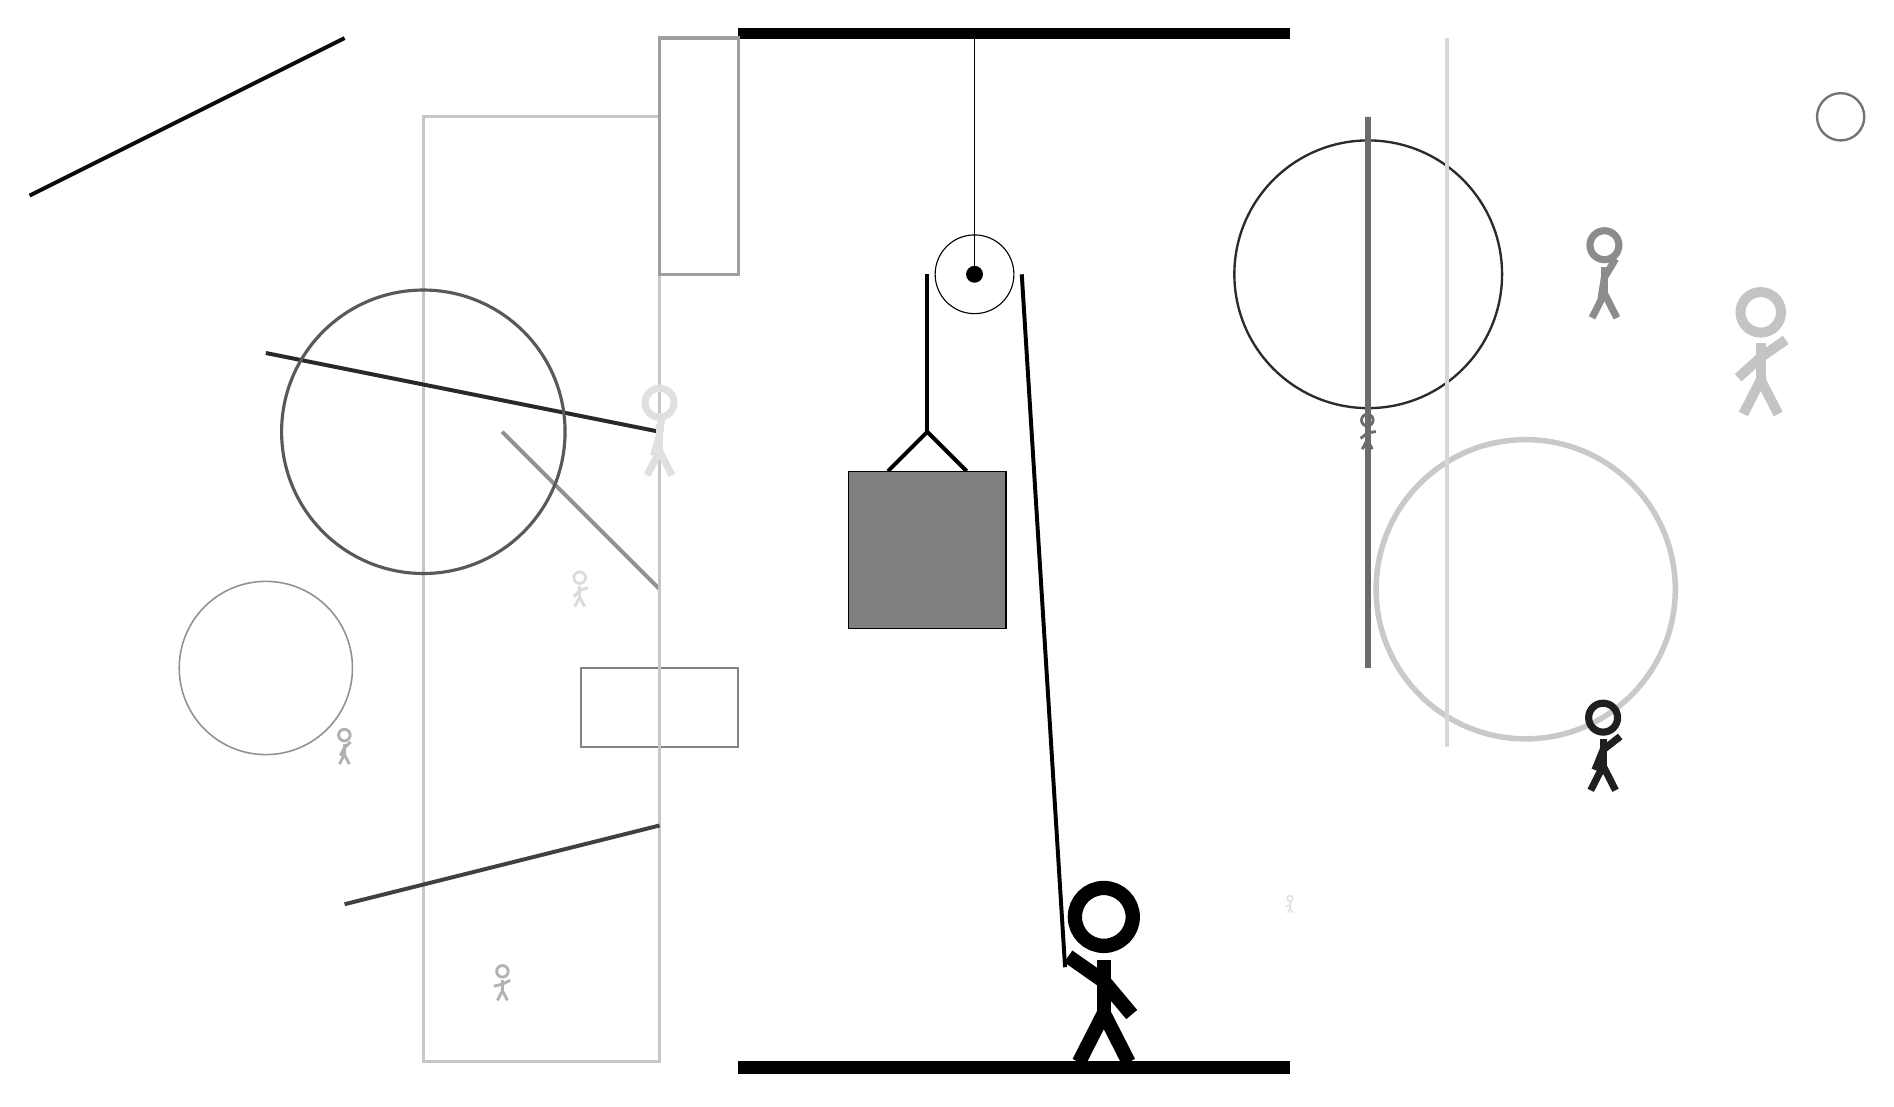
\begin{tikzpicture}
		%%%%% START %%%%%
		
		\draw[fill=black] (-2, 10) rectangle (5, 10.125);
		
		\node[line width=0.3mm, color=black!23] at (11, 6) {\Strichmaxerl[7][42][35]};
		
		\draw[line width=0.5mm, color=black!43](-3, 3) -- (-5, 5);
		\node[line width=0.7mm, color=black!14] at (-4, 3) {\Strichmaxerl[2][47][19]};
		\draw[line width=0.5mm, color=black!96](-7, 10) -- (-11, 8);
		\draw[line width=0.3mm, color=black!49] (-2, 2) rectangle (-4, 1);
		\draw[line width=0.4mm, color=black!22] (-3, -3) rectangle (-6, 9);
		\node[line width=0.7mm, color=black!31] at (-7, 1) {\Strichmaxerl[2][62][44]};
		\draw [line width=0.3mm, color=black!83](6, 7) circle (1.7);
		\node[line width=0.4mm, color=black!30] at (-5, -2) {\Strichmaxerl[2][13][27]};
		
		\draw[line width=0.5mm, color=black!84](-3, 5) -- (-8, 6);
		\draw [line width=0.3mm, color=black!55](12, 9) circle (0.3);
		
		\node[line width=0.4mm, color=black!45] at (9, 7) {\Strichmaxerl[5][81][59]};
		\draw [line width=0.2mm, color=black!43](-8, 2) circle (1.1);
		
		\node[line width=0.4mm, color=black!58] at (6, 5) {\Strichmaxerl[2][39][10]};
		\node[line width=0.6mm, color=black!12] at (5, -1) {\Strichmaxerl[1][20][77]};
		\node[line width=0.3mm, color=black!12] at (-3, 5) {\Strichmaxerl[5][74][83]};
		
		\draw [line width=0.7mm, color=black!21](8, 3) circle (1.9);
		\draw[line width=0.4mm, color=black!38] (-2, 7) rectangle (-3, 10);
		\draw [line width=0.4mm, color=black!65](-6, 5) circle (1.8);
		\draw[line width=0.7mm, color=black!58] (6, 2) rectangle (6, 9);
		\draw[line width=0.4mm, color=black!16] (7, 1) rectangle (7, 10);
		
		\node[line width=0.2mm, color=black!88] at (9, 1) {\Strichmaxerl[5][68][38]};
		\draw[line width=0.5mm, color=black!75](-3, 0) -- (-7, -1);
		
		\draw (1, 7) circle (0.5);
		\draw[fill=black] (1, 7) circle (0.1);
		\draw (1, 10) -- (1, 7);
		
		\draw[line width=0.5mm] (-0.1, 4.5) -- (0.4, 5.0) -- (0.9, 4.5);
		\draw[fill=black!50] (-0.6, 4.5) rectangle (1.4, 2.5);
		
		\draw[line width=0.5mm] (0.4, 7) -- (0.4, 5.0);
		\centerarc[line width=0.5mm](1, 7)(0:180:0.6);
		\draw[line width=0.5mm](1.6, 7) -- (2.15, -1.8);
		
		\node at (2.6, -1.9) {\Strichmaxerl[10][-35][-50]};
		
		\draw[fill=black] (-2, -3) rectangle (5, -3.15);
		
		%%%%% END %%%%%
	\end{tikzpicture}
\end{document}